% arara: pdflatex
% arara: bibtex
% arara: pdflatex
% arara: pdflatex
\documentclass[12pt]{article}
\usepackage{amsmath}
\usepackage{graphicx}
\usepackage{hyperref}
\usepackage{textcomp}
\usepackage[section]{placeins}
\usepackage{hhline}
\usepackage{float}
\usepackage{caption} 
\usepackage{enumitem}

\captionsetup[table]{skip=10pt}

\bibliographystyle{acm}

\hypersetup{
  colorlinks, linkcolor=red
}

\begin{document}


\title{CS838 Project Final Report}
\author{Sek Cheong}
\maketitle

\begin{abstract}
This project is an attempt to build a deep convolutional neural network (CNN) to colorize gray scale images whiteout user intervention. We frame the colorization model as a regression with the intensity component of an image as input and predict the color components of that image.  We use a pre-trained model, VGG16~\cite{VGG16}, to extract features that will be used for training our colorizing model.
\end{abstract}

\section{Introduction}
Colorization of gray scale images is a relative simple task for human to perform, yet it a quite challenging problem to solve by machine learning algorithms. To colorize an image, a human only needs to recall that the sky is blue, trees are green. For many objects, a human can apply some imagination to colorize an gray scale images relative well. However, it is a difficult task for computer to solve, in that it is obvious to a human that an apple cannot be blue. But for a machine learning algorithm, if it has not seen enough apple examples before, it could color an apple blue or green or a number of different color as long as the cost function defined for the learning algorithm returns similar values for a number of different colors. It is beyond the scope of this project to design a model that can perform at a similar level of human in colorization. We aim to explorer process of colorization using CNN and use the transfer learning technique to help improve our colorization CNN. 

We frame the colorization problem as an regression problem. We build an CNN that accepts an gray scale image and predicts the color components of the image. We then combine the gray scale and color components to form an predicted color image as show in Figure 1. We start with a VGG16 pre-trained model, which is designed for image classification purposes, and we modify the model for image colorization.   

\begin{figure}[!ht]
 \centering
  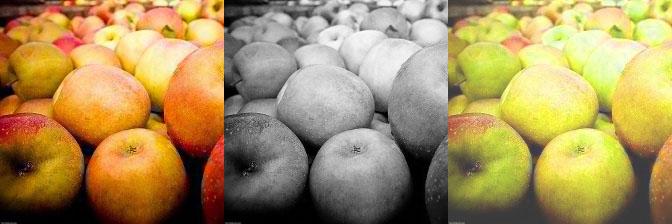
\includegraphics[width=4.0in]{resource/example.jpg}
 \label{sampleimages}
 \caption{The picture on the left is the ground truth, the picture in the middle is the input, and the picture on the right is the pridected color image.}
\end{figure}


\section{Related Work}
Our project was primarily motivated by Ryan Dahl's Automatic Colorization~\cite{RYAN2016} blog post. Ryan proposed a model which utilize a concept of hypercolumns~\cite{HYPERCOL}. A hypercolumn for a pixel in the input image is a vector of all the activations above that pixel. The Ryan implemented this was by forwarding an image through the VGG network and then extracting a few layers, upscaling them to the original image size, and concatenating them all together. As shown by Zeiler and Fergus~\cite{Zeiler} a lot of useful information were represented in the intermediate layers of a CNN, therefore intermediate layers of a classification network can provide useful information for colorization.

Zhang et al., Larsson et al.~\cite{Zhang}  and Iizuka et al.~\cite{Iizuka} have developed similar but much more sophisticated colorization systems. The systems differ primary in their CNN architectures and loss functions. While Zhang et al., use a classification loss, with rebalanced rare classes, Larsson et al. use an un-rebalanced classification loss, and Iizuka et al. use a regression loss.


\section{Approach}

\subsection{Data Set}
There are a number of data sets for computer vision available publicly. Among the available image data sets the ImageNet data set is the most famous one. Many machine learning models involving vision are trained on ImageNet images. There are approximately one million image files from $1000$ categories in the ImageNet data set and it is about $120$G in size. We downloaded (took really long time!) the entire image set and looked some images. It turned that there are many images either in black and white or were not useful coloring examples. We believe a good coloring example image should contain a single object, the foreground and background should be distinguishable and should have good saturation and hue. It would be impossible to hand pick the good examples given the time constrain and the shear number of images in the data set. For this reason we switched to MIRFLICKR~\cite{MIR08} which is a collection of images from the flicker picture sharing website. The MIRFLICKR pictures are very appearing visually because, unlike ImageNet, these pictures are produced by flicker users with the intention for human consumption.  

We picked the first $10000$ images (black and white images were excluded) from MIRFLICKR as our image set. The images was then split into $70\%$ for training, $20\%$ for tuning, and the remaining $10\%$ for testing. 

\begin{figure}[!ht]
 \centering
  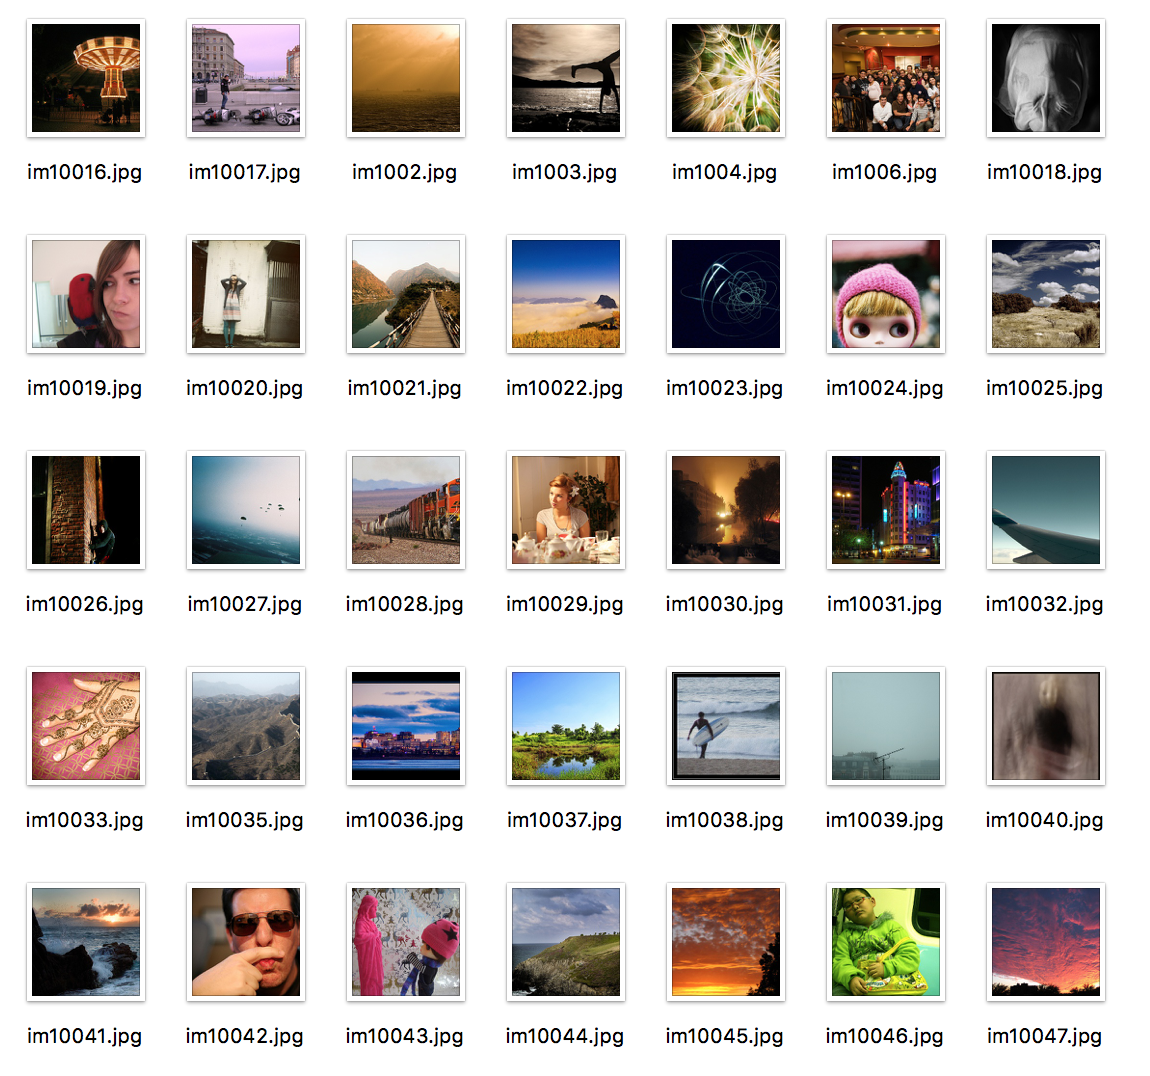
\includegraphics[width=4.0in]{resource/exampleimages.png}
 \label{sampleimages}
 \caption{Some sample images from our training set}
\end{figure}



\subsection{Data Preprocessing}
The images were come in various sizes but for out model we use accepts images of $224\times224$ pixels. The rational for choosing such image size was because the images trained on VGG16 were $224\times224$ pixels and we would use VGG16 weights for training our own model. To make the MIRFLICKR images compatible with our model we need to resize the images into $224\times224$ pixels. However, instead of simply resizing the images into $224\times224$ pixels, we scale the shorter side of the image to $224$ pixels and crop the image along with the $224$ pixel side to  $224\times224$ pixels. We think training on images with the correct aspect ration might give a better result for coloring. The scaling and cropping was done by a python script~\cite{PYDATA} we created.

To construct a training example from a color image we could convert the image into gray scale image and use the gray scale image as input $\boldsymbol{X}$, and the RGB values as the target $\boldsymbol{Y}$. Note, the input is a $1\times224\times224$ vector and the target is a $3\times224\times224$ vector. As explained by Ryan Dahl\textquotesingle s web blog post~\cite{RYAN2016} that we could convert the image from RGB color space into YUV color space, where Y is the intensity of the image, and UV are two chrominance components of the image. This reduces the target vector $\boldsymbol{Y}$ to $2\times224\times224$. The following figure shows the original image, the Y component, the U component, and the V component. 

\begin{figure}[!ht]
 \centering
  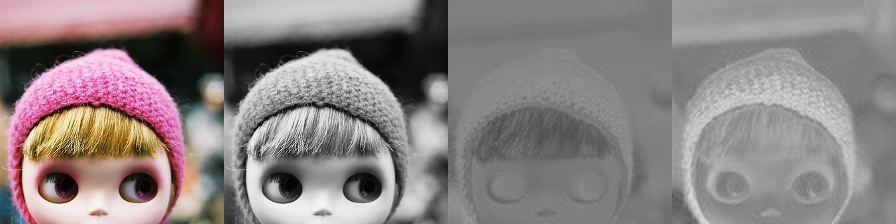
\includegraphics[width=5.0in]{resource/YUV.png}
 \label{yuvimage}
 \caption{The original picture and its YUV components}
\end{figure}


\subsection{The Model}
We use the VGG16 model as our starting model as shown in Figure 3. The VGG16 has an output layer of $1000$ units with Softmax activation. The output layer is designed in such a way that it can be used to classify image from a thousand categories. Our initial design of transfer learning was that after loading the weights for the model we remove the final layer and replace with a $2\times224\times224$ regression unit. For activation function we use the hyperbolic tangent function. This proved to be a disaster as the number of parameters in the model skyrocketed to $545,402,688$! from  $138,357,544$. 


\begin{figure}[H]
 \centering
  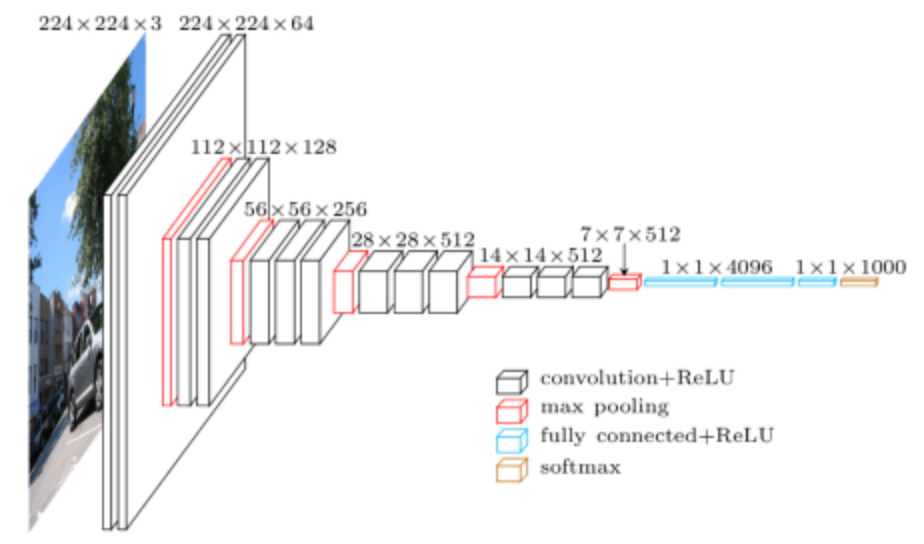
\includegraphics[width=5.0in]{resource/vgg16.png}
\center
\label{fig:vggvis}
 \caption{The VGG16 model visualization}
\end{figure}

It turns out that YUV color space is closely related YCbCr color space which was used for digital encoding of color information suited for video and still-image compression and transmission such as MPEG and JPEG~\cite{YUVWIKI}. For our use we could simply treat UV as same as CbCr. The main difference between these two color spaces was scaling. Since we scale pixel values between $-1$ and $1$, it wouldn't make any difference for us. The nice property of YCbCr color space was that human eyes are far more sensitive to change in intensity than color. This allowed us to throw away most of the CbCr information while still maintain the image quality. The process of throwing away color information is called color space compression. 

We experimented around different compression rate and it appeared that we can throw away $80\%$ of the color information and the image still maintains very good color quality. 


\begin{figure}[H]
 \centering
  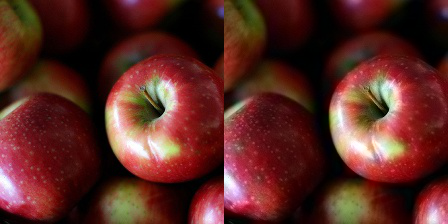
\includegraphics[width=5.0in]{resource/colorcompress.png}
 \label{yuvimage}
 \caption{Image on the left with $90\%$ color space compression}
\end{figure}

As show in the figure above, the image on the left is the original image, the image on the right has $90\%$ of the color information removed.

We started out with a off-the-shelf VGG16 model. We removed the last three layers of the network these are two fully connected layers and one soft max activation layer. 

We discarded $85\%$ of the color information, that is we resize the chrominance components UV to $15\%$ of its original size using bi-cubic interpolation. This process reduced the UV size down to $33\times33$ from $224\times224$. This gave us the output dimension of $33\times33\times2=2178$. 

We added the following layers to the VGG model:

\begin{table}[H]
	\caption{The additional layers added to VGG16 for colorization}
  	\centering
	\begin{tabular}{|l|l|r|}
		\hline 
		dropout 1 (Droupput)          &  (None, 25088)          &    0           \\ \hline
		fc1 (Dense)                   &  (None, 1536)           &    38536704    \\ \hline
        leaky ReLu 1 (LeakyReLU)      &  (None, 1536)           &    0           \\ \hline
        dropout 2 (Dropout)           &  (None, 1536)           &    0           \\ \hline
        fc2 (Dense)                   &  (None, 1536)           &    2360832     \\ \hline
        leaky relu 2 (LeakyReLU)      &  (None, 1536)           &    0           \\ \hline
        dropout 3 (Dropout)           &  (None, 1536)           &    0           \\ \hline
        batch normalization 1 (Batch  &  (None, 1536)           &    6144        \\ \hline
        fc3 (Dense)                   &  (None, 2178)           &    3347586     \\ \hline
        colorize (Activation)         &  (None, 2178)           &    0           \\ \hline 
	\end{tabular}
\end{table}


We adjusted the output layer to the size of reduced color dimension. The new model has $58,962,882$ parameters. This is significantly fewer parameters than the original VGG16 and our initial model.


\begin{table}[H]
	\caption{The colorize model (with color space compression) based on VGG16 architecture}
  	\centering
	\begin{tabular}{|l|l|r|}
		\hline 
		Layer (type)                  &  Output Shape           &    Parameters  \\ \hhline{|=|=|=|}
		input 1 (Input Layer)         &  (None, 224, 224, 3)    &    0           \\ \hline
		block 1 conv 1 (Conv 2D)      &  (None, 224, 224, 64)   &    1792        \\ \hline 
		block 1 conv 2 (Conv 2D)      &  (None, 224, 224, 64)   &    36928       \\ \hline 
		block 1 pool (Max Pooling 2D) &  (None, 112, 112, 64)   &    0           \\ \hline 
		block 2 conv 1 (Conv 2D)      &  (None, 112, 112, 128)  &    73856       \\ \hline 
		block 2 conv 2 (Conv 2D)      &  (None, 112, 112, 128)  &    147584      \\ \hline 
		block 2 pool (Max Pooling 2D) &  (None, 56, 56, 128)    &    0           \\ \hline 
		block 3 conv 1 (Conv 2D)      &  (None, 56, 56, 256)    &    295168      \\ \hline 
		block 3 conv 2 (Conv 2D)      &  (None, 56, 56, 256)    &    590080      \\ \hline 
		block 3 conv 3 (Conv 2D)      &  (None, 56, 56, 256)    &    590080      \\ \hline 
		block 3 pool (Max Pooling 2D) &  (None, 28, 28, 256)    &    0           \\ \hline 
		block 4 conv 1 (Conv 2D)      &  (None, 28, 28, 512)    &    1180160     \\ \hline 
		block 4 conv 2 (Conv 2D)      &  (None, 28, 28, 512)    &    2359808     \\ \hline 
		block 4 conv 3 (Conv 2D)      &  (None, 28, 28, 512)    &    2359808     \\ \hline 
		block 4 pool (Max Pooling 2D) &  (None, 14, 14, 512)    &    0           \\ \hline 
		block 5 conv 1 (Conv 2D)      &  (None, 14, 14, 512)    &    2359808     \\ \hline 	
		block 5 conv 2 (Conv 2D)      &  (None, 14, 14, 512)    &    2359808     \\ \hline 
		block 5 conv 3 (Conv 2D)      &  (None, 14, 14, 512)    &    2359808     \\ \hline 
		block 5 pool (Max Pooling 2D) &  (None, 7, 7, 512)      &    0           \\ \hline 
		flatten (Flatten)             &  (None, 25088)          &    0           \\ \hline 
		dropout 1 (Droupput)          &  (None, 25088)          &    0           \\ \hline
		fc1 (Dense)                   &  (None, 1536)           &    38536704    \\ \hline
        leaky ReLu 1 (LeakyReLU)      &  (None, 1536)           &    0           \\ \hline
        dropout 2 (Dropout)           &  (None, 1536)           &    0           \\ \hline
        fc2 (Dense)                   &  (None, 1536)           &    2360832     \\ \hline
        leaky relu 2 (LeakyReLU)      &  (None, 1536)           &    0           \\ \hline
        dropout 3 (Dropout)           &  (None, 1536)           &    0           \\ \hline
        batch normalization 1 (Batch  &  (None, 1536)           &    6144        \\ \hline
        fc3 (Dense)                   &  (None, 2178)           &    3347586     \\ \hline
        colorize (Activation)         &  (None, 2178)           &    0           \\ \hline 
	\end{tabular}
\end{table}


\subsection{Training}
The computing resource used for training this model is a MacPro Quad Core computer with a 3.5Gh Quad CPU and 16G of memory. We attempted to run the model on the GPU of the computer but GPU did not have the minimum required memory for run the model. 


We trained our model with $1500$ images with $50$ epoch, the training set is probably not large enough to train a complex task such as colorization, but due to the limited computing resources and time constrain, we had to settle with $1500$ samples. The training process took about $25$ hours to complete. We used the standard SGD learning algorithm and use Mean Square Root (MSE) as our loss function. The learning of between $0.01 and 0.05$, momentum of $0.9$ and weight decay of $4e-5$ tend to work the best. 

We tried Euclidean distance between colors as lossy function. This doesn't seem to make much difference. We also tried absolute difference between colors as lossy function and it turned out not work as well as MSE. The source~\cite[PYCODE] code is available at GitHub.


\section{Results and Discussion}

\begin{figure}[H]
 \centering
  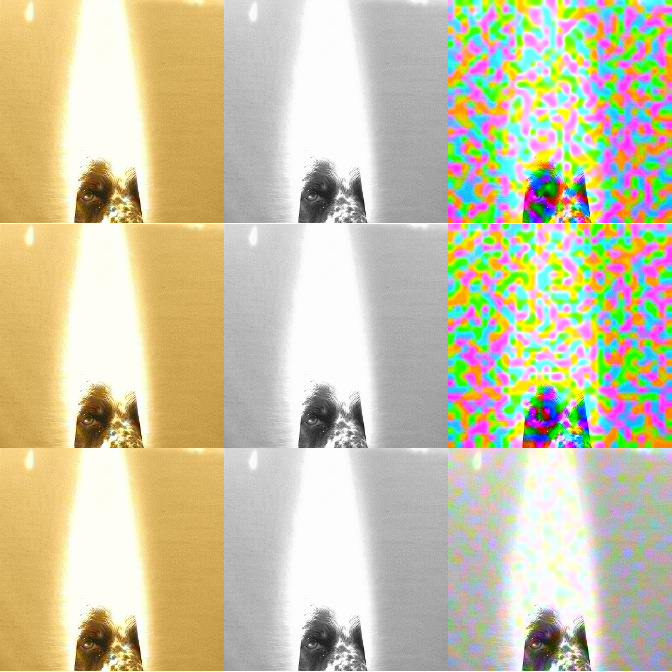
\includegraphics[width=5.0in]{resource/trainstage.png}
 \label{yuvimage}
 \caption{Predictions in various epoch, left the ground truth, middle the input image, right the predicted image}
\end{figure}


Here are some predicted images after running 50 epochs on the model
\begin{figure}[H]
 \centering
 \includegraphics[width=5.0in]{resource/im25.jpg}
\end{figure}


\begin{figure}[H]
 \centering
 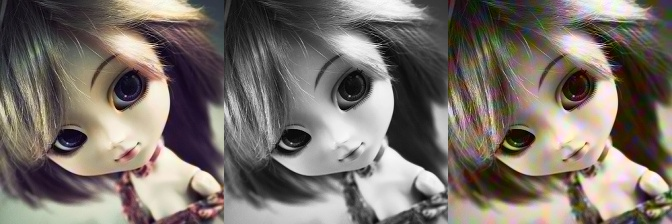
\includegraphics[width=5.0in]{resource/im43.jpg}
\end{figure}


\begin{figure}[H]
 \centering
 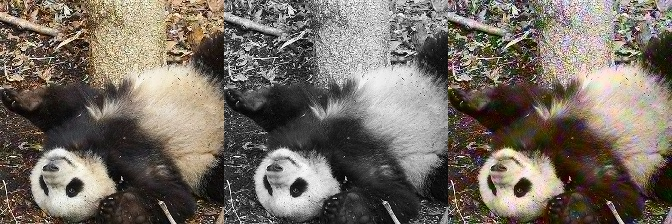
\includegraphics[width=5.0in]{resource/im89.jpg}
\end{figure}


\begin{figure}[H]
 \centering
 \includegraphics[width=5.0in]{resource/im94.jpg}
\end{figure}



The model did not do quite as we as we expected. There are slight tints of green for grass and tree but other than that we get low saturation sepia tone in most of coloring objects. More training probably will not increase the quality of colorization significantly. We speculated this is probably due to the loss function we used. The MSE returns an every error for the prediction which might explain why most of the output has the sepia mid tone look. 

Unlike image classification, colorization is a muitlmodal regression problem. The model should predict a color on each pixel or a patch of neighboring pixels. Instead of predicting each pixel values. It might be helpful that we encode the final fully connected layer as patches of $15\times15$ images and concatenated them together to form a one denominational vector. We then add another layer to just predict the color of each patches and up convert the out patches to the input image size to form a predicted image.

We tried to build a histogram distribution of colors in the sample and predicted images then use the Kullback Leibler divergence as the loss function. Unfortunately, were unable to make it work in Tensorflow an Kersa. The build-in fixed\_histogram function in Tensorflow will return none which caused Keras to crash. We asked the problem in various online forum with no avail.

Using transfer learning with pre-trained VGG16 weights did help produce better result. We trained our model from scratch and after 50 epochs the output images were still very nosy. We believe the semantic feature learned in the pooling layers in the VGG16 are useful for colorization as well. 



\section{Future Work}
\begin{enumerate}
	\item Trying out classification instead of regression might improve the results for some classes.
	\item Replace VGG16 with a more modern classification model like ResNet~\cite{ResNet}. More layers and more training could improve the colorization results. 
\item  The problem with averaging loss which resulted low saturated sepia tone is a major impediment for colorization problem. We need to modeling the loss better. The Generative Adversarial Networks~\cite{GAN} seem like a promising solution. 
\end{enumerate}


\section{Conclusion}
In this project we experiment a basic technique for image colorization using CNN using extracted feature from pre-trained VGG16 network. While our colorization scheme show some evidence of working, to build auto colorization model that produce color image at the level that is good enough for human consumption is still quite a distance away. We created the frame work for learning colorization using Tensorflow and Keras. This frame work can be used to experiment with some more advanced colorization systems described in  ~\cite{Zhang}~\cite{Iizuka}~\cite{Guillaume}.


\bibliography{biblio}

\end{document}